\section{List Mode Data Analysis}
	For data collected using a digitizer, or similiar equipment, this menu features numerous options to analyze and save various data. This has the expectation of time dependent data being collected, i.e. a source is being pulsed using a logic pulse. With detector and sync pulse data both being captured and recoreded as raw data.
		\subsection{View Time Decay}
			This is used to generate a plot of multiple region of interest pulse arrival times relative to the sync pulse. This must be run after having used the list mode data set of tools. The first pop up will request the number of data sets to be plotted. After selection of this, the windows file explorer will be generated. It will expect a file that is two columns, the first being time stamps, the second being a number of counts accumulated during the time step. This will be repeated for the total number of files selected. Several additional windows will appear that request additional information regarding the frequency, duty cylce, and location of region dividers. All of which are optional. The data will be processed and plotted in the window upon clicking the ``Process'' button. A high quality image, 600dpi, can be saved with the selection of the ``Save Image'' button.

	\subsection{Analyze List Mode Data}
		This is the primary interface for loading and manipulating time dependent data. As such an entire section is dedicated to this later in this document.
		
	\subsection{Detection Probability}
		\subsubsection{Theory}
		This is used to determine the time required to reach 99\% detection probability. Poisson and Gaussian Statistics are implemented in their respsective regimes, less than 30 counts for Poisson and any number of counts greater than 30 for Gaussian. For Poisson statistics, the distribution is only dependent on the mean, $\mu$, in this case the mean is taken as the number of counts, this is seen in equation \ref{eq:poisson}. Gaussian statistic distribution is dependent on a mean, $\mu$, and variance, the mean is again taken to be the number of counts and the standard deviation to be $\sigma=\sqrt{N}$, the distribution function is seen in equation \ref{eq:gaussian}.

	\begin{equation}
		P=\frac{\mu^kexp\left(-\mu\right)}{k!}
		\label{eq:poisson}
	\end{equation}
	\begin{equation}
		P=\frac{1}{2\pi\sigma^2}exp\left(\frac{\left(\mu-k\right)^2}{2\sigma^2}\right)
		\label{eq:gaussian}
		\end{equation}
	An example of a foreground and background distribution plotted together are seen in Figure \ref{fig:pdf}. The background distribution is used in conjunction with a maximum false alarm rate, one alarm per eight hours is the default, to find a threshold to be used to determine the detection probability. \\
	
	\begin{figure}[h!]
		\centering
		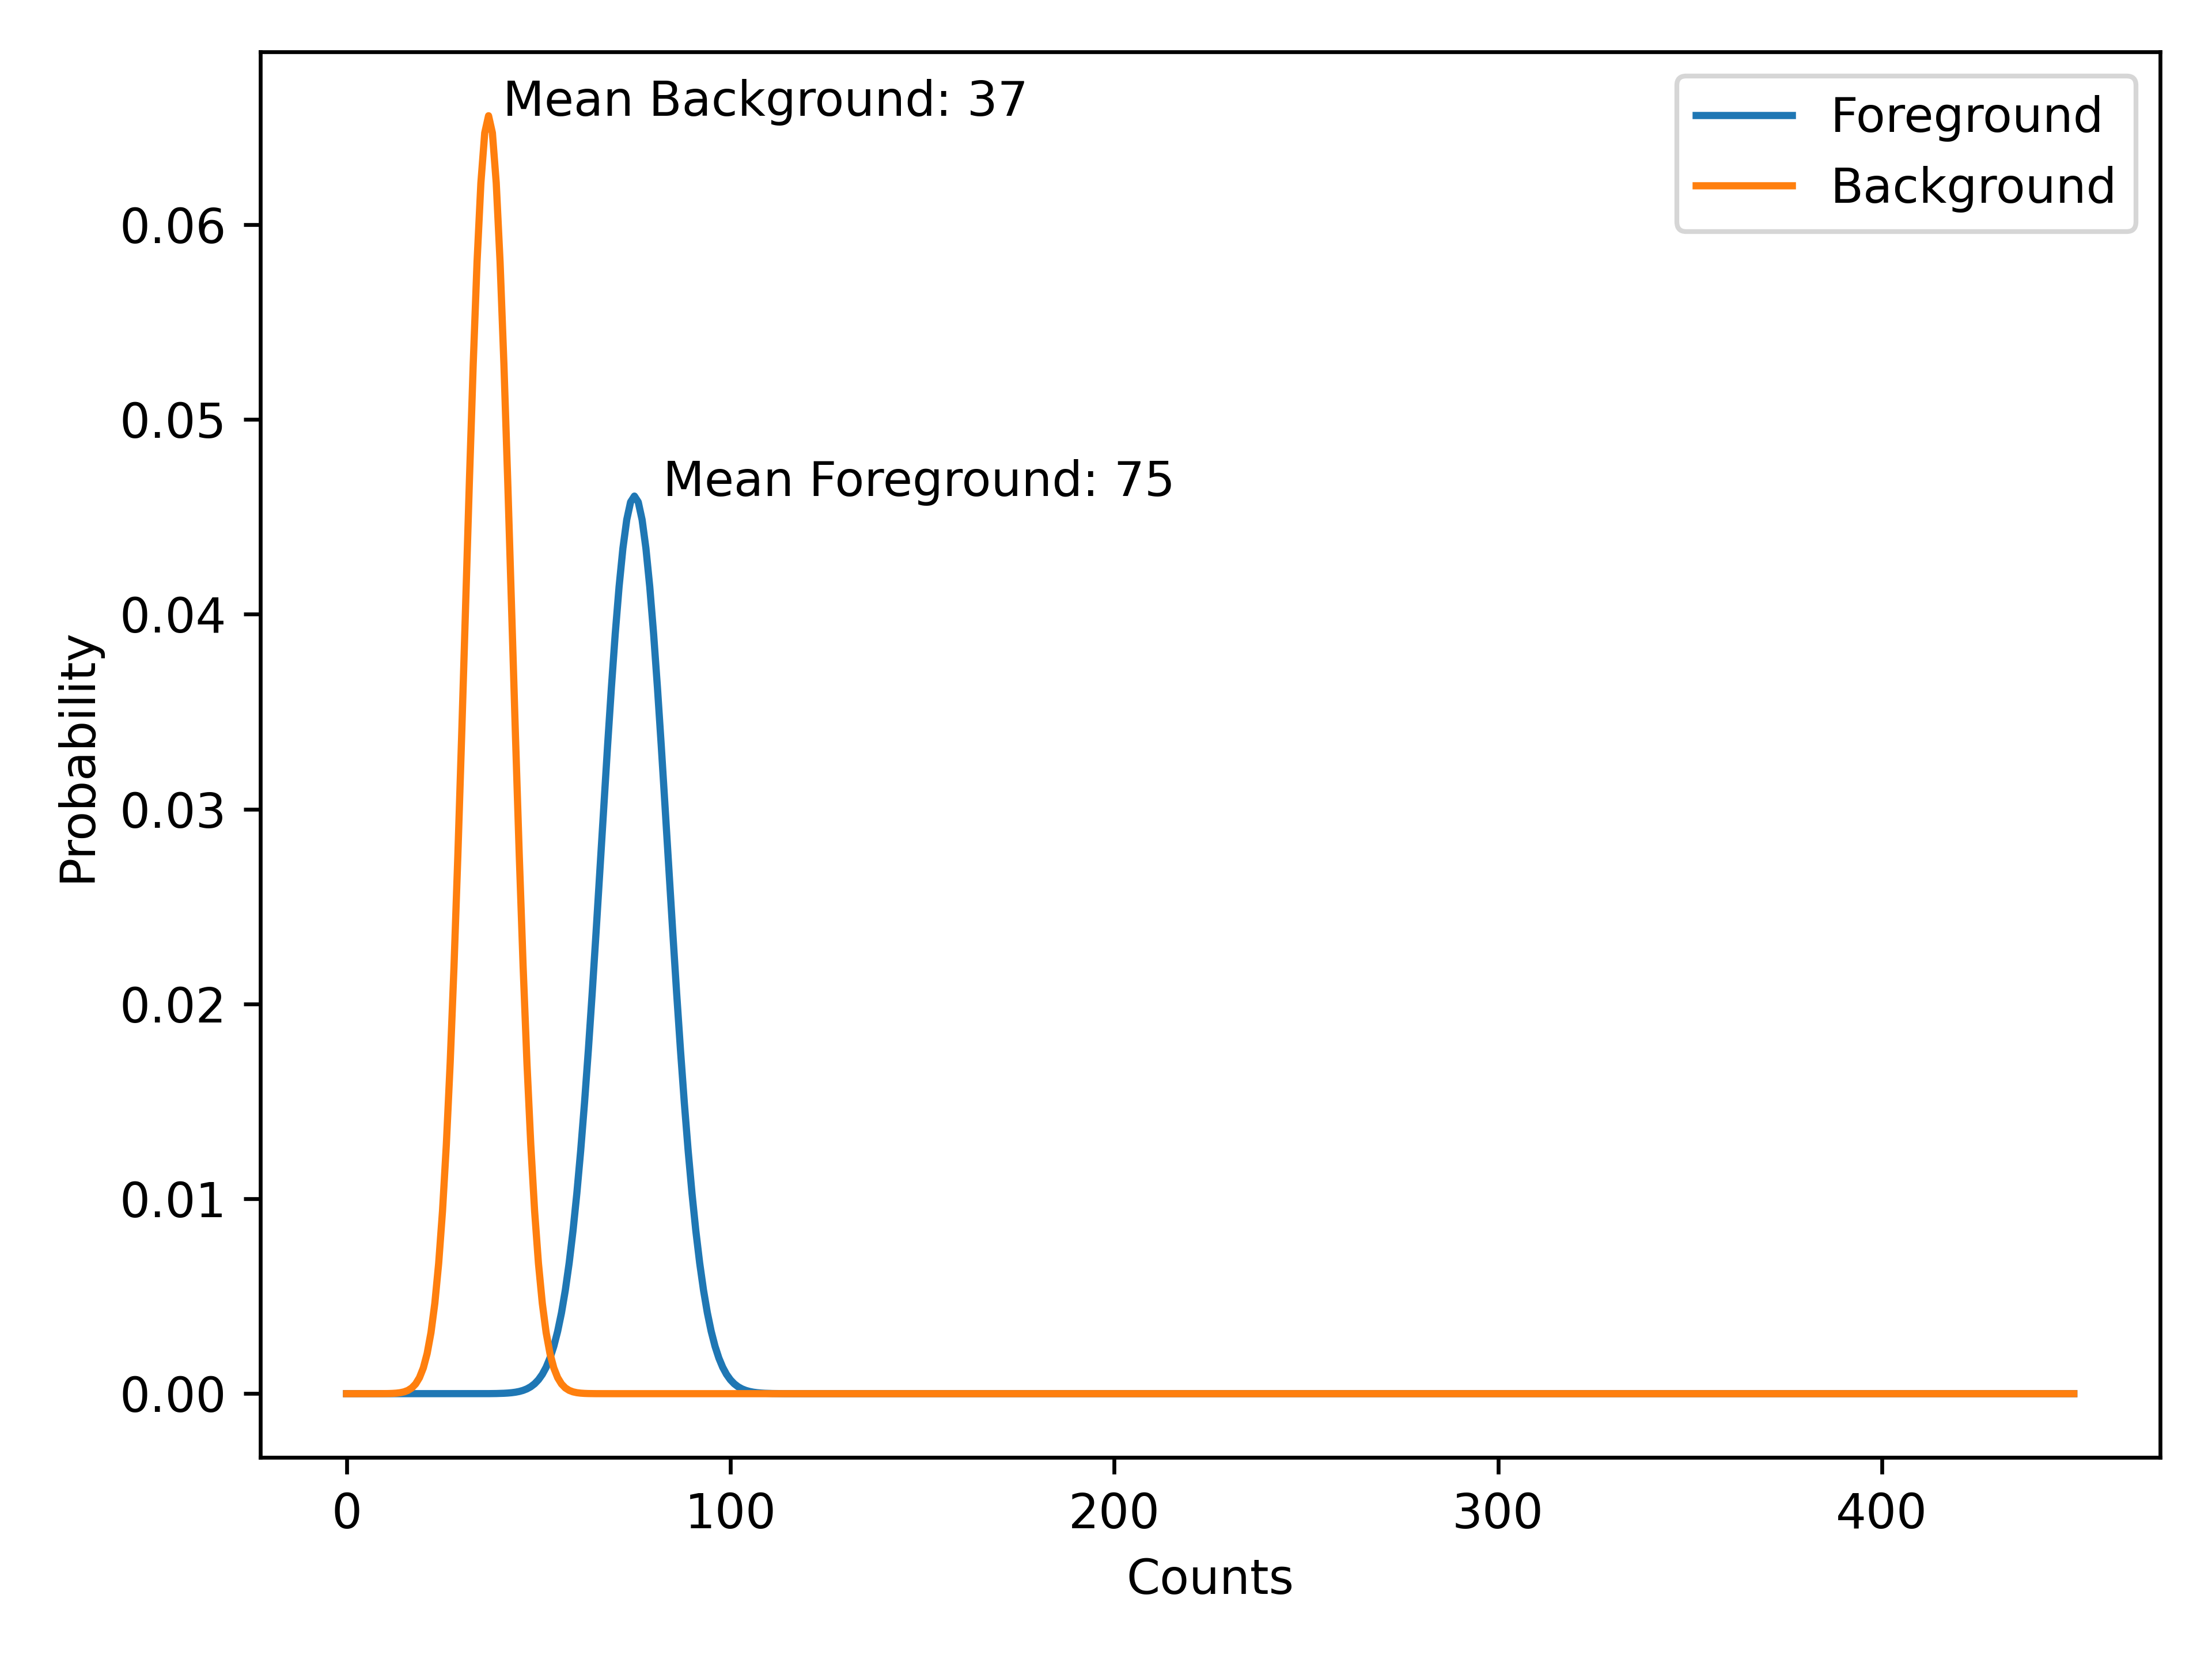
\includegraphics[width=0.6\linewidth]{pdf.png}
		\caption{Probability distribution functions for a foreground and background plotted together.}
		\label{fig:pdf}
	\end{figure}
	The probability distribution functions are then numerically integrated using trapeziodal rule. The integration of this must sum to exactly one. The foreground and background cumulative density functions, along with the threshold is seen in Figure \ref{fig:cdf}.\\
	\begin{figure}[h!]
		\centering
		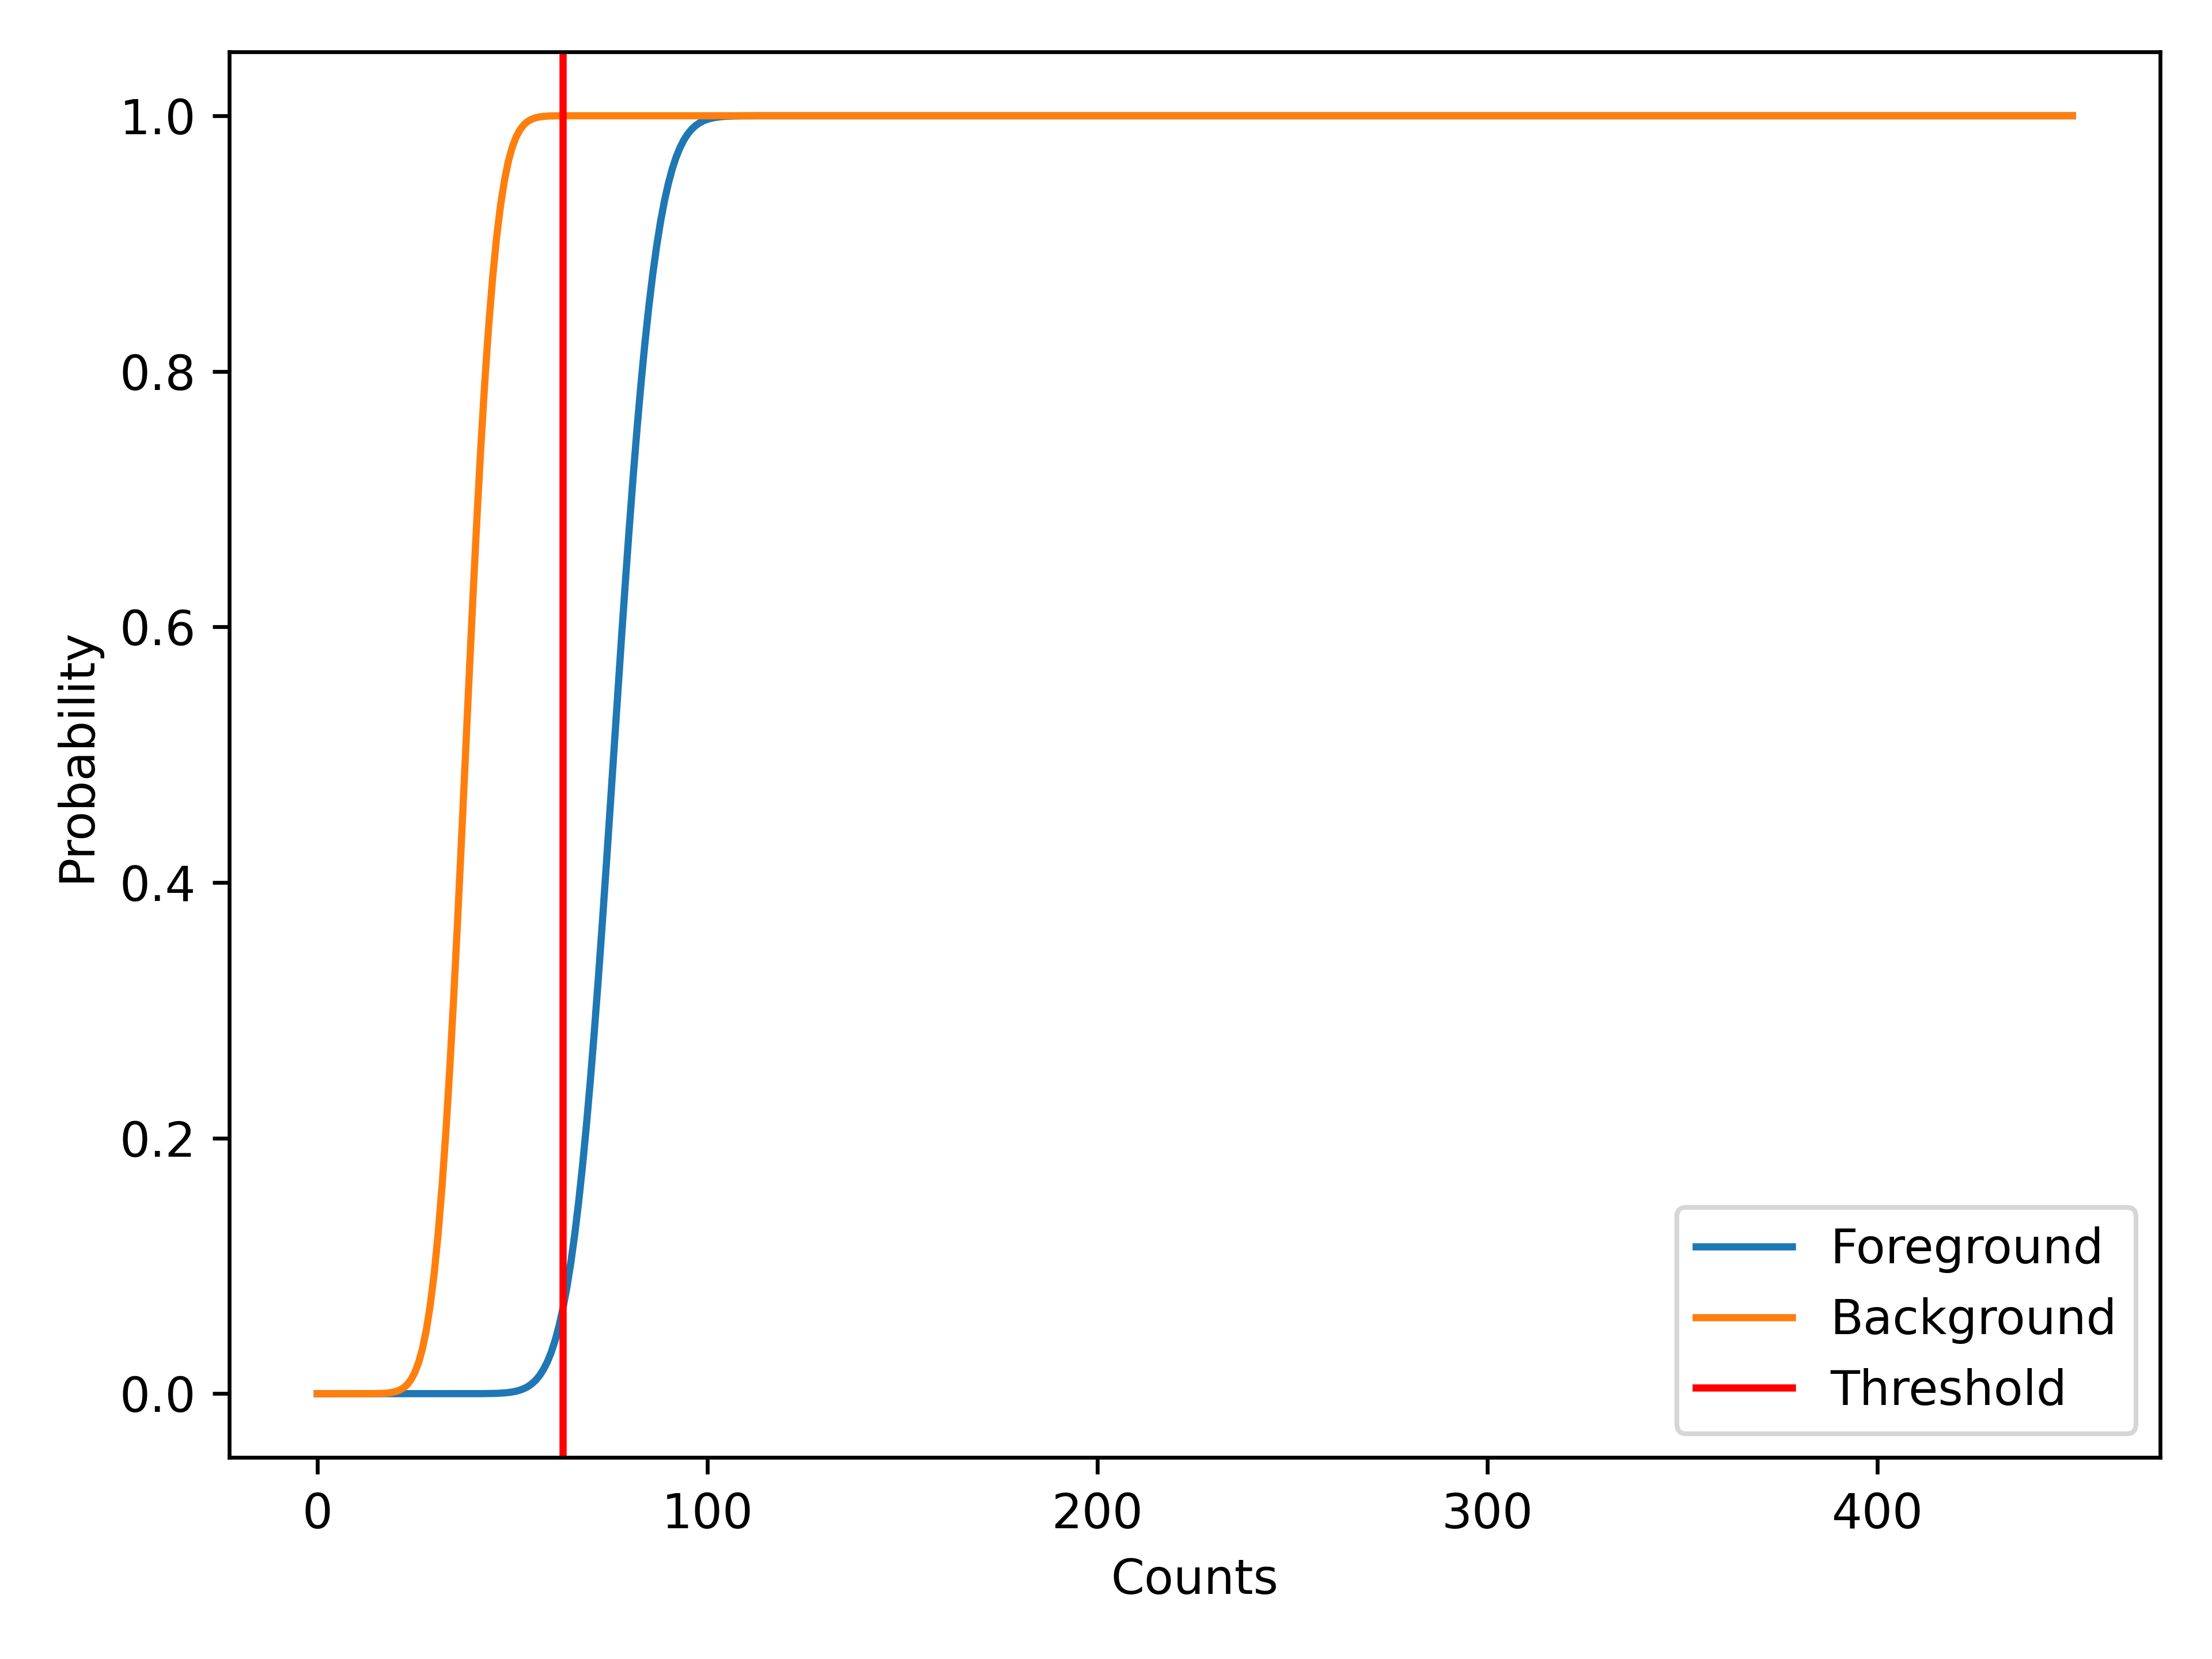
\includegraphics[width=0.6\linewidth]{cdf.png}
		\caption{Cummulative density function with detection threshold indicated.}
		\label{fig:cdf}
	\end{figure}
Using the cummulative density function and the threshold, the detection probability is found as $1-f_{cdf}$ where $f_{cdf}$ is the foreground cummulative density function evaluated at the threshold index. For the given examples the detection probability is 93\%. 
\subsubsection{Implementation}
	Two files are required for this to work, a background and a foreground, these are selected in this order. The files are generated using the ``Save ROI'' method in the ``List Mode Reader'' interface. The files take a two column form with a time of arrival and energy as the two columns. A window will appear to set the first time step to begin integrating. This is due to statistical fluctuations at extremely low count fields. A total of 181 time steps are taken over the entire length of the accumulated time.\\ 
	
It should be noted that this portion may take a significant portion of time to run due to have to generate, and integrate 362 discrete functions. \\

Upon completeion of the analysis, the software will automatically bring up a windows file explorer to save the data points out, to be used for generation of a video. This will then generate a plot of the probability of detection versus time, the software will indicate the point at which the detection probability rises above 99\% for the first time. Care should be taken by the user to ensure the start point has not removed prudent data, but is high enough to remove any erroneous data points. 

\subsection{Save Probability Video}
	This generates a video from the probability data saved using the detection probability function. It expects as input a two column file with time in the first column and a detection probability in the second. It saves as an mp4 file type.



